\UC{Registrazione}
\begin{figure}[H]
    \centering
    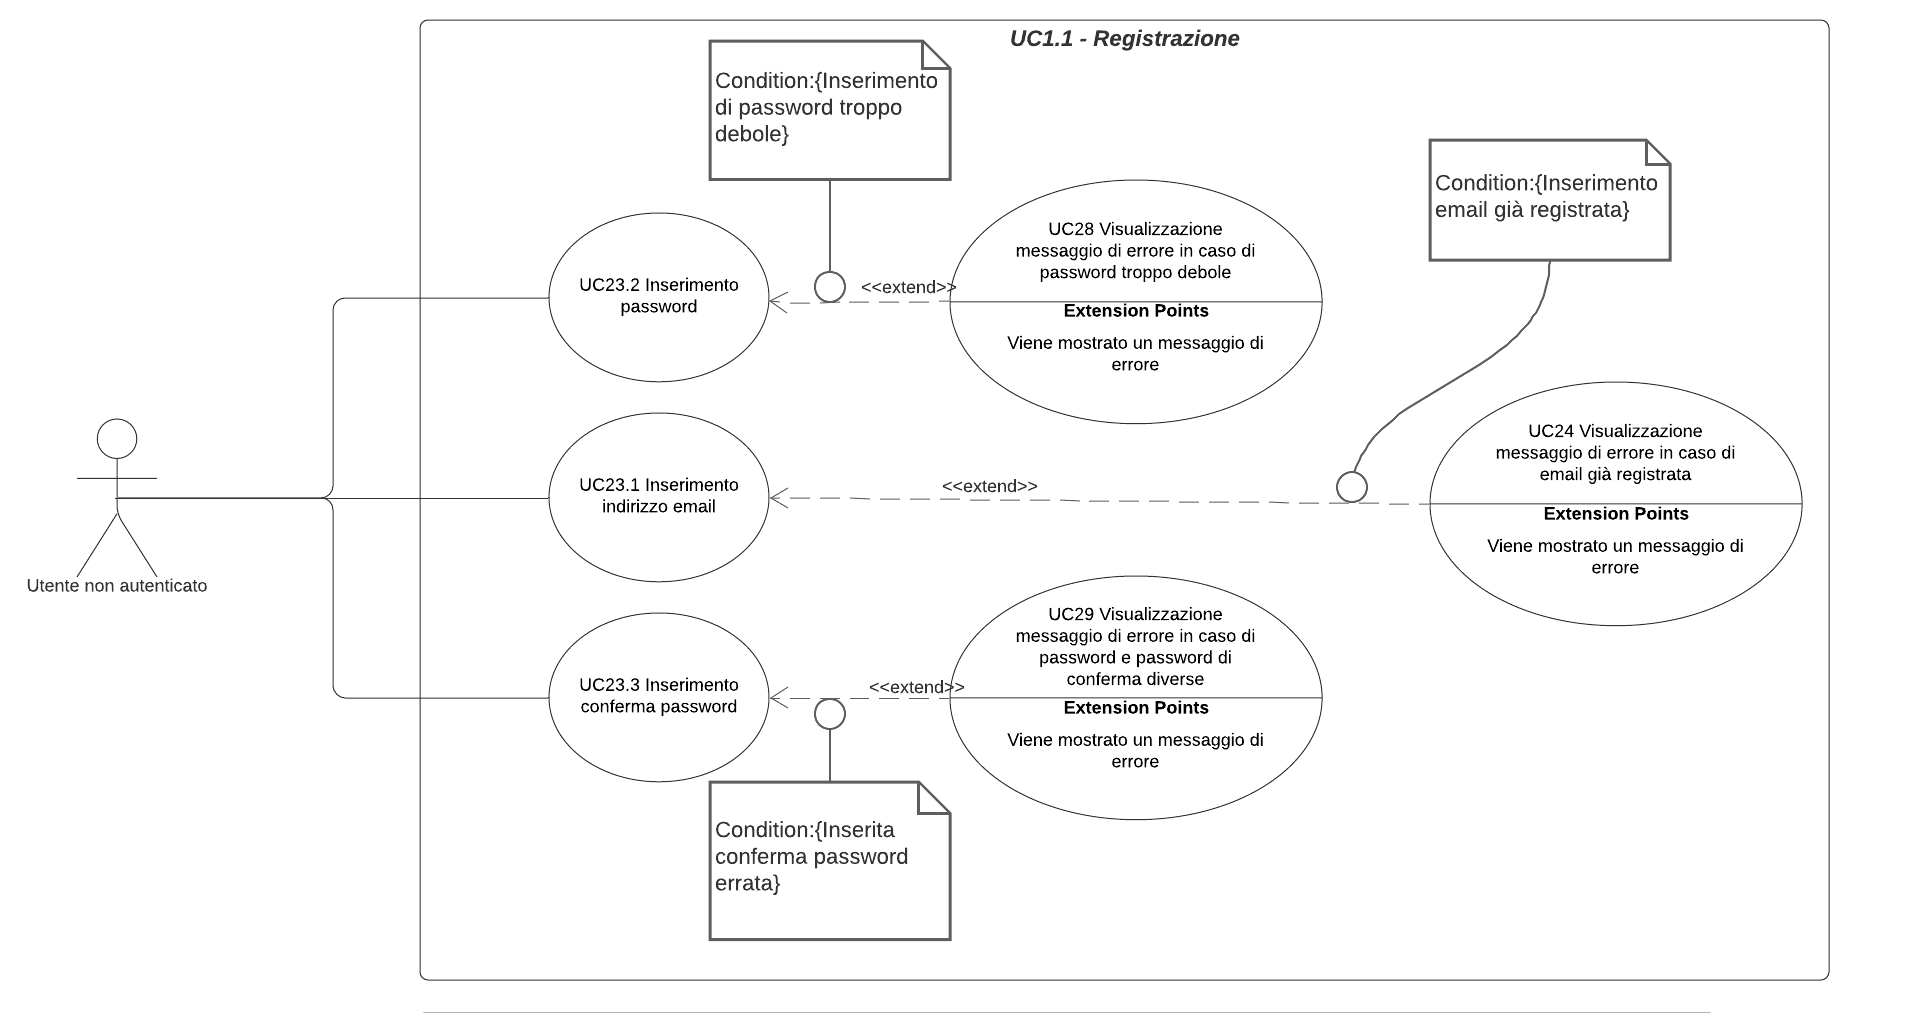
\includegraphics[scale=0.6]{Immagini/DiagrammiUC/UC1.1Registrazione}
    \caption{Diagramma di \actualUC: Registrazione}
    \label{fig:RegistrazionePiattaforma}
\end{figure}

L'utente non autenticato che non dispone di credenziali può registrarsi e accedere come acquirente nella piattaforma usando l'email e la password.
\begin{itemize}
    \item \textbf{Attori primari:} utente non autenticato;
    \item \textbf{Precondizione:} l'utente non è ancora presente nella piattaforma e si trova nella schermata di registrazione;
    \item \textbf{Postcondizione:} l'utente è registrato con un account acquirente ed è autenticato come tale sulla piattaforma;
    \item \textbf{Scenario principale:} l'utente crea un account compilando tutti i campi del modulo di registrazione nel seguente modo:
    \begin{itemize}
    	\item (UC) - Inserimento nome;
    	\item (UC) - Inserimento cognome;
        \item (UC) - Inserimento indirizzo e-mail per la registrazione;
        \item (UC) - Inserimento password per la registrazione;
        \item Inserimento conferma password;
        \item L'utente non autenticato conferma il proprio indirizzo email inserito per la registrazione;
        \item L'utente non autenticato richiede la registrazione.
    \end{itemize}
	\item \textbf{Scenario alternativo:} l'utente inserisce un indirizzo email già presente nella piattaforma
	\begin{itemize}
		\item (UC Estensione) - Viene mostrato un messaggio d'errore indirizzo email già registrato nella piattaforma;
		\item L'utente non può procedere all'autenticazione.
	\end{itemize}
	\item \textbf{Scenario alternativo:} l'utente compila i campi dati per la password e la conferma della stessa con due password diverse
	\begin{itemize}
		\item (UC Estensione) - Viene mostrato un messaggio d'errore campi dati password e conferma password diversi;
		\item L'utente non può procedere all'autenticazione.
	\end{itemize}
	%\item \textbf{Scenario alternativo:} l'utente prova ad eseguire l'operazione di registrazione senza aver compilato alcun campo dati del modulo per eseguire la registrazione;
    \item \textbf{Estensioni:}
    \begin{itemize}
        \item (UC) - Visualizzazione messaggio di errore in caso di email già registrata nella piattaforma;
        \item (UC) - Visualizzazione messaggio di errore in caso di campi dati obbligatori non compilati;
        %\item (UC) - Visualizzazione messaggio di errore in caso di modulo non compilato;
        \item (UC) - Visualizzazione messaggio di errore in caso di password e password di conferma diverse.
    \end{itemize}
	\item \textbf{Inclusioni:}
	\begin{itemize}
		\item (UC) - Inserimento del nome per la registrazione;
		\item (UC) - Inserimento del cognome per la registrazione; 
		\item (UC) - Inserimento indirizzo email per la registrazione;
		\item (UC) - Inserimento password per la registrazione.
	\end{itemize}
\end{itemize}

\subUC{Inserimento del nome per la registrazione}
\begin{itemize}
	\item \textbf{Attori primari:} utente non autenticato;
	\item \textbf{Precondizione:} l'utente non è autenticato;
	\item \textbf{Postcondizione:} l'utente ha inserito il proprio nome;
	\item \textbf{Scenario principale:} l'utente non autenticato inserisce il proprio nome per la registrazione;
	\item \textbf{Scenario alternativo:} l'utente non inserisce il cognome, in questo caso:
	\begin{itemize}
		\item (UC Estensione) - Viene mostrato un messaggio d'errore campo dati obbligatorio non inserito;
		\item L'utente non può procedere con la registrazione.
	\end{itemize}
	\item \textbf{Estensioni:}
	\begin{itemize}
		\item (UC) - Visualizzazione messaggio campo dati obbligatorio non inserito.
	\end{itemize}
\end{itemize}

\subUC{Inserimento del cognome per la registrazione}
\begin{itemize}
	\item \textbf{Attori primari:} utente non autenticato;
	\item \textbf{Precondizione:} l'utente non è autenticato;
	\item \textbf{Postcondizione:} l'utente ha inserito il proprio cognome;
	\item \textbf{Scenario principale:} l'utente non autenticato inserisce il proprio cognome per la registrazione;
	\item \textbf{Scenario alternativo:} l'utente non inserisce il cognome, in questo caso:
	\begin{itemize}
		\item (UC Estensione) - Viene mostrato un messaggio d'errore campo dati obbligatorio non inserito;
		\item L'utente non può procedere con la registrazione.
	\end{itemize}
	\item \textbf{Estensioni:}
	\begin{itemize}
		\item (UC) - Visualizzazione messaggio campo dati obbligatorio non inserito.
	\end{itemize}
\end{itemize}

\subUC{Inserimento indirizzo email per la registrazione}
L'utente non autenticato inserisce l'indirizzo email.
\begin{itemize}
	\item \textbf{Attori primari:} utente non autenticato;
	\item \textbf{Precondizione:} l'utente non autenticato non ha ancora fornito un'email ed ha a disposizione un campo dati dove inserirla;
	\item \textbf{Postcondizione:} l'utente non autenticato ha fornito un indirizzo email valido;
	\item \textbf{Scenario principale:} l'utente non autenticato inserisce il proprio indirizzo email per procedere con la registrazione;
	\item \textbf{Scenario alternativo:} l'utente non inserisce l'email:
	\begin{itemize}
		\item (UC Estensione) - Viene mostrato un messaggio d'errore campo dati obbligatorio non inserito;
		\item L'utente non può procedere con la registrazione.
	\end{itemize}
	\item \textbf{Scenario alternativo:} l'utente non autenticato ha inserito un indirizzo email con un formato non corretto, in questo caso
	\begin{itemize}
		\item (UC Estensione) - Viene mostrato un messaggio d'errore indirizzo email non rispetta il formato;
		\item L'utente non può procedere con la registrazione.
	\end{itemize}
	\item \textbf{Estensione:}
	\begin{itemize}
		\item (UC) - Visualizzazione messaggio campo dati obbligatorio non inserito;
		\item (UC) - Visualizzazione messaggio di errore in caso di email non valida.
	\end{itemize}
\end{itemize}

\subUC{Inserimento password per la registrazione}
L'utente non autenticato inserisce una password.
\begin{itemize}
	\item \textbf{Attori primari:} utente non autenticato;
	\item \textbf{Precondizione:} l'utente non autenticato non ha ancora fornito una password che rispetta i requisiti di complessità ed ha a disposizione un campo dati dove inserirla;
	\item \textbf{Postcondizione:} l'utente ha inserito una password valida.
	\item \textbf{Scenario principale:} l'utente non autenticato inserisce una password che rispetti le condizioni imposte per procedere con la registrazione;
	\item \textbf{Scenario alternativo:} l'utente non inserisce la password:
	\begin{itemize}
		\item (UC Estensione) - Viene mostrato un messaggio d'errore campo dati obbligatorio non inserito;
		\item L'utente non può procedere con la registrazione.
	\end{itemize}
	\item \textbf{Scenario alternativo:} l'utente non autenticato ha inserito una password con un formato non corretto, in questo caso:
	\begin{itemize}
		\item (UC) - Viene mostrato un messaggio d'errore password che non rispetta i requisiti di complessità;
		\item L'utente non procede con la registrazione.
	\end{itemize}
	\item \textbf{Estensione:}
	\begin{itemize}
		\item (UC) - Visualizzazione messaggio campo dati obbligatorio non inserito;
		\item (UC) - Visualizzazione messaggio di errore in caso di password troppo debole.
	\end{itemize}
\end{itemize}

\UC{Autenticazione nella piattaforma con credenziali venditore}
\begin{figure}[H]
    \centering
    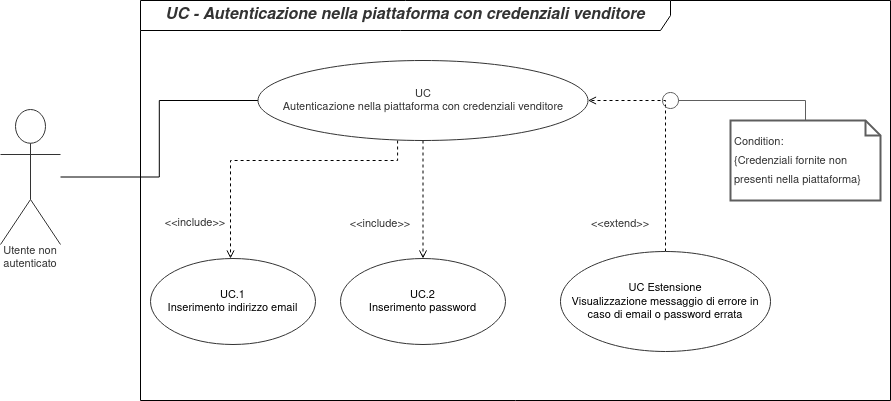
\includegraphics[scale=0.6]{Immagini/DiagrammiUC/AccessoVenditore.png}
    \caption{Diagramma di \actualUC: Autenticazione nella piattaforma con credenziali venditore} 
    \label{fig:LoginVenditore}
\end{figure}

L'utente non autenticato che dispone di credenziali venditore può accedere nella piattaforma usando l'email e la password.
\begin{itemize}
    \item \textbf{Attori primari:} utente non autenticato;
    \item \textbf{Precondizione:} l'utente dispone di credenziali venditore e si trova nella schermata di login;
    \item \textbf{Postcondizione:} l'utente è autenticato come venditore e si trova sulla \glo{dashboard};
    \item \textbf{Scenario principale:} l'utente accede alla piattaforma con delle credenziali in questo modo:
    \begin{itemize}
        \item (UC) - Inserimento indirizzo email;
        \item (UC) - Inserimento password;
        \item Richiede l'autenticazione;
        \item L'utente è autenticato come venditore;
        \item L'utente viene portato alla dashboard.
    \end{itemize}
	\item \textbf{Scenario alternativo:} l'utente compila i campi dati con delle credenziali
	\begin{itemize}
		\item Inserimento indirizzo email;
		\item Inserimento password;
        \item Richiede l'autenticazione.
    \end{itemize}
	Ma le credenziali fornite non appartengono alla piattaforma, quindi:
	\begin{itemize}
		\item (UC Estensione) - Viene visualizzato un messaggio di errore credenziali non presenti nella piattaforma;
		\item L'utente rimane non autenticato e alla schermata di login.
	\end{itemize}
    \item \textbf{Estensioni:}
    \begin{itemize}
        \item (UC) - Visualizzazione messaggio di errore in caso di credenziali errate.
    \end{itemize}
    \item \textbf{Inclusioni:}
    \begin{itemize}
    	\item (UC) - Inserimento indirizzo email;
    	\item (UC) - Inserimento password.
    \end{itemize}
\end{itemize}

\resetSubUC
\subUC{Inserimento indirizzo email per l'autenticazione}
\begin{itemize}
	\item \textbf{Attori primari:} utente non autenticato;
	\item \textbf{Precondizione:} l'utente dispone di credenziali venditore e si trova nella schermata di login;
	\item \textbf{Postcondizione:} l'utente ha inserito il proprio indirizzo email;
	\item \textbf{Scenario principale:} l'utente non autenticato inserisce l'indirizzo email per l'autenticazione.
	\item \textbf{Scenario alternativo:} l'utente non inserisce l'email:
	\begin{itemize}
		\item (UC) - Viene mostrato un messaggio d'errore;
		\item L'utente non può procedere all'autenticazione.
	\end{itemize}
	\item \textbf{Estensioni:}
	\begin{itemize}
		\item (UC) - Visualizzazione messaggio campo dati obbligatorio non inserito.
	\end{itemize}
\end{itemize}

\subUC{Inserimento password per l'autenticazione}
\begin{itemize}
	\item \textbf{Attori primari:} utente non autenticato;
	\item \textbf{Precondizione:} l'utente dispone di credenziali venditore e si trova nella schermata di login;
	\item \textbf{Postcondizione:} l'utente ha inserito la propria password;
	\item \textbf{Scenario principale:} l'utente non autenticato inserisce la password per l'autenticazione;
	\item \textbf{Scenario alternativo:} l'utente non inserisce la password:
	\begin{itemize}
		\item (UC) - Viene mostrato un messaggio d'errore campo dati obbligatorio non inserito;
		\item L'utente non può procedere all'autenticazione.
	\end{itemize}
	\item \textbf{Estensioni:}
	\begin{itemize}
		\item (UC) - Visualizzazione messaggio campo dati obbligatorio non inserito.
	\end{itemize}
\end{itemize}

\UC{Autenticazione nella piattaforma con credenziali acquirente}
\begin{figure}[H]
	\centering
	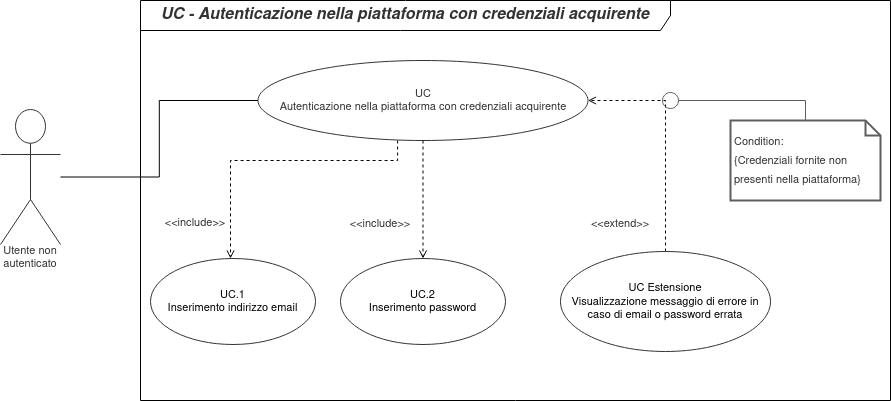
\includegraphics[scale=0.6]{Immagini/DiagrammiUC/AccessoAcquirente.png}
	\caption{Diagramma di \actualUC: Autenticazione nella piattaforma con credenziali acquirente} 
	\label{fig:LoginAcquirente}
\end{figure}

L'utente non autenticato che dispone di credenziali acquirente può accedere nella piattaforma usando l'email e la password.
\begin{itemize}
	\item \textbf{Attori primari:} utente non autenticato;
	\item \textbf{Precondizione:} l'utente dispone di credenziali acquirente e si trova nella schermata di login;
	\item \textbf{Postcondizione:} l'utente è autenticato come acquirente e si trova nella schermata principale;
	\item \textbf{Scenario principale:} l'utente accede alla piattaforma con delle credenziali in questo modo:
	\begin{itemize}
		\item (UC) - Inserimento indirizzo email venditore;
		\item (UC) - Inserimento password;
		\item Richiede l'autenticazione;
		\item L'utente è autenticato come acquirente;
		\item L'utente viene portato alla schermata principale.
	\end{itemize}
	\item \textbf{Scenario alternativo:} l'utente compila i campi dati con delle credenziali
	\begin{itemize}
		\item (UC) - Inserimento indirizzo;
		\item (UC) - Inserimento password;
		\item Richiede l'autenticazione.
	\end{itemize}
	Ma le credenziali fornite non appartengono alla piattaforma, quindi:
	\begin{itemize}
		\item (UC Estensione) - Viene visualizzato un messaggio di errore credenziali non presenti nella piattaforma;
		\item L'utente rimane non autenticato e alla schermata di login.
	\end{itemize}
	\item \textbf{Estensioni:}
	\begin{itemize}
		\item (UC) - Visualizzazione messaggio di errore in caso di credenziali errate.
	\end{itemize}
	\item \textbf{Inclusioni:}
	\begin{itemize}
		\item (UC) - Inserimento indirizzo email;
		\item (UC) - Inserimento  password. 
		\end{itemize}
\end{itemize}

\UC{Password dimenticata}
\begin{figure}[H]
    \centering
    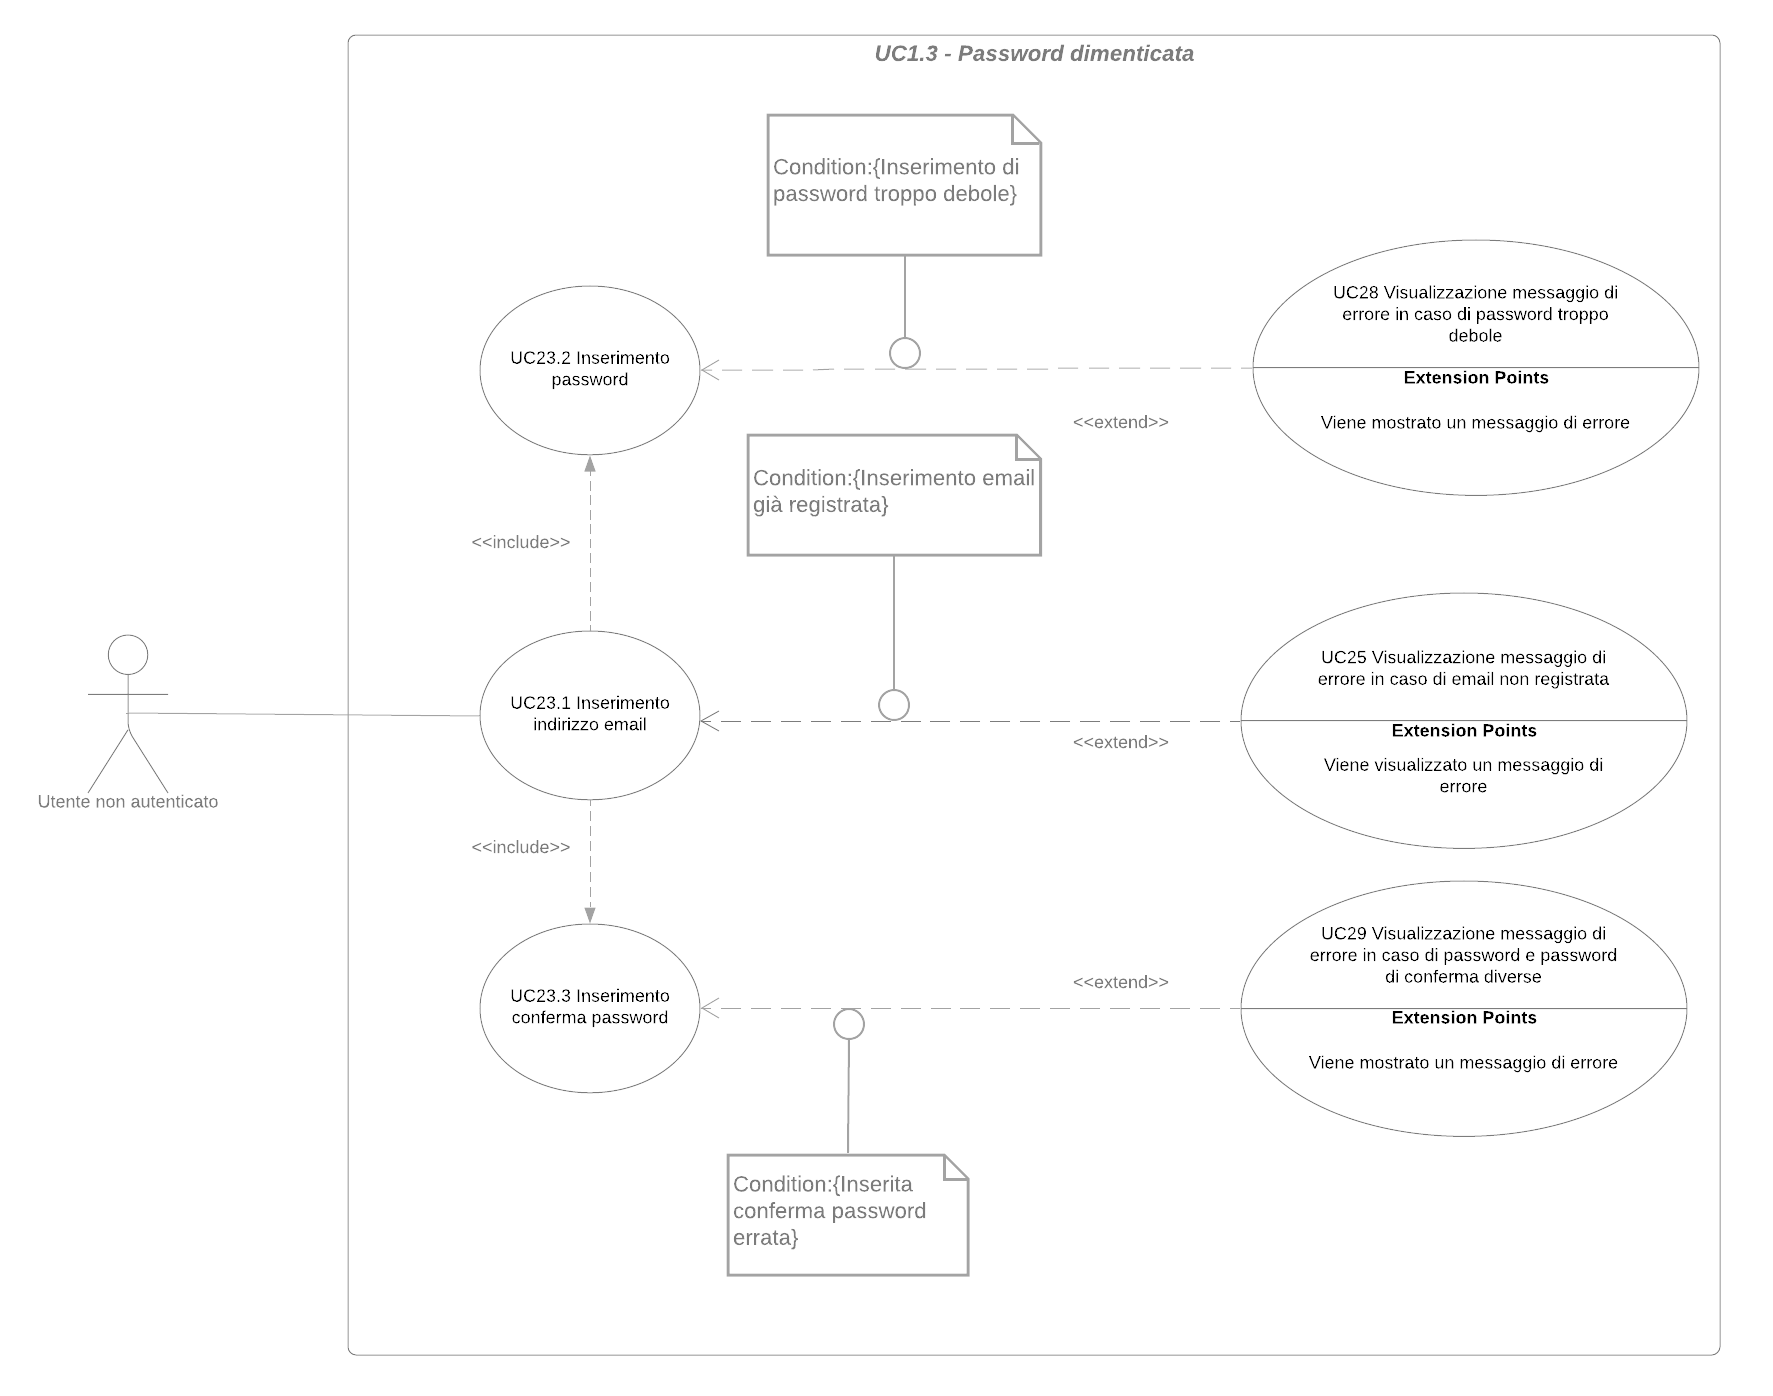
\includegraphics[scale=0.2]{Immagini/DiagrammiUC/UC1.3PasswordDimenticata.png}
    \caption{Diagramma di \actualUC: Password dimenticata} 
    \label{fig:PasswordDimenticata}
\end{figure}

L'utente che dispone di credenziali si è dimenticato la propria password e la vuole cambiare.
\begin{itemize}
    \item \textbf{Attori primari:} utente non autenticato;
    \item \textbf{Precondizione:} l'utente non autenticato che dispone di credenziali si trova nella schermata per cambiare la password;
    \item \textbf{Postcondizione:} l'utente è autenticato e ha cambiato la password con cui poter effettuare l'accesso alla piattaforma;
    \item \textbf{Scenario principale:} l'utente che dispone di credenziali si è dimenticato la propria password e per cambiarla deve compiere i seguenti passi:
    \begin{itemize}
        \item (UC) - Inserimento indirizzo email;
        \item Invio link per il cambio della password all'indirizzo email indicato;
        \item Apertura della schermata per il cambio della password;
        \item (UC) - Inserimento nuova password;
        \item Inserimento conferma nuova password;
        \item L'utente è autenticato e ha cambiato la password.
    \end{itemize}
	\item \textbf{Scenario alternativo:} l'utente compila i campi dati
	\begin{itemize}
		\item (UC) - Inserimento indirizzo email.
	\end{itemize}
	Ma l'indirizzo email non appartiene alla piattaforma, quindi:
	\begin{itemize}
		\item (UC Estensione) - Viene visualizzato un messaggio di errore indirizzo email non registrato nella piattaforma;
		\item L'utente rimane non autenticato e alla schermata di login.
	\end{itemize}
	\item \textbf{Scenario alternativo:} l'utente compila i campi dati
	\begin{itemize}
		\item (UC) - Inserimento indirizzo email;
		\item Invio link per il cambio della password all'indirizzo email indicato;
		\item Apertura della schermata per il cambio della password;
		\item (UC Estensione) - Inserimento nuova password;
		\item Inserimento conferma nuova password;
	\end{itemize}
	Ma la password inserita non rispetta i requisiti di complessità, quindi:
	\begin{itemize}
		\item (UC Estensione) - Viene visualizzato un messaggio di errore password che non rispetta i requisiti di complessità;
		\item L'utente rimane non autenticato e alla schermata di login. 
	\end{itemize}
    \item \textbf{Estensioni:}
    \begin{itemize}
        \item (UC) - Visualizzazione messaggio di errore in caso di email non registrata;
        \item (UC) - Visualizzazione messaggio di errore in caso di password e password di conferma diverse.
    \end{itemize}
    \item \textbf{Inclusioni:}
    \begin{itemize}
        \item (UC) - Inserimento nuova password.
    \end{itemize}
\end{itemize}

\UC{Logout dalla piattaforma}
L'utente autenticato decide di scollegarsi dalla piattaforma.
\begin{itemize}
    \item \textbf{Attori primari:} utente autenticato;
    \item \textbf{Precondizione:} l'utente ha eseguito il login precedentemente e vuole scollegarsi dalla piattaforma;
    \item \textbf{Postcondizione:} l'utente autenticato diventa un utente non autenticato;
    \item \textbf{Scenario principale:} l'utente autenticato decide di scollegarsi dalla piattaforma e compie l'azione di scollegamento.
\end{itemize}